\documentclass[tikz,border=8pt]{standalone}
% Shared look for every TikZ diagram. Load with \input{../../tools/tikz-style.tex}
\usepackage[T1]{fontenc}
\usepackage{lmodern}
\renewcommand{\sfdefault}{lmr}  % diagrams use the same serif as the text
\usetikzlibrary{arrows.meta, positioning, shapes.geometric, calc, fit, backgrounds}
\definecolor{cblue}{HTML}{4C78A8}
\definecolor{corange}{HTML}{F58518}
\definecolor{cgreen}{HTML}{54A24B}
\definecolor{cred}{HTML}{E45756}
\definecolor{cpurple}{HTML}{B279A2}
\definecolor{cgrey}{HTML}{6B6B6B}
\tikzset{
  every picture/.style={font=\sffamily, line width=1.2pt},
  box/.style={draw=#1, fill=#1!12, rounded corners=4pt, align=center, inner sep=7pt, minimum height=1.1cm},
  box/.default=cgrey,
  arrow/.style={-{Stealth[length=3mm]}, draw=cgrey, line width=1.4pt},
  title/.style={font=\sffamily\bfseries\Large},
  note/.style={font=\sffamily\small, text=cgrey, align=center},
}
\AtBeginDocument{\hyphenpenalty=10000 \exhyphenpenalty=10000}

\begin{document}
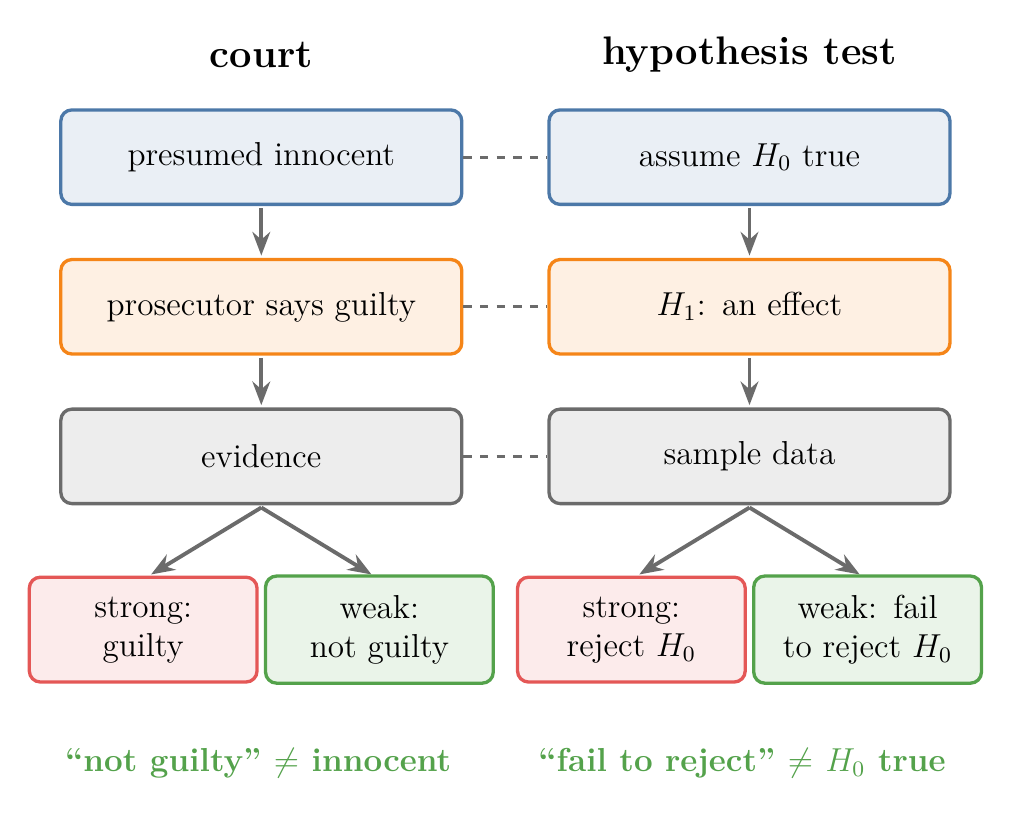
\begin{tikzpicture}[every node/.append style={font=\sffamily\large}, b/.style={box=#1, text width=4.6cm, minimum height=1.2cm}]
  \node[title] at (0,1.3) {court};
  \node[title] at (6.2,1.3) {hypothesis test};
  \foreach \y/\c/\a/\b in {0/cblue/{presumed innocent}/{assume $H_0$ true},
                           -1.9/corange/{prosecutor says guilty}/{$H_1$: an effect},
                           -3.8/cgrey/{evidence}/{sample data}} {
    \node[b=\c] (l) at (0,\y) {\a};
    \node[b=\c] (r) at (6.2,\y) {\b};
    \draw[cgrey, dashed, line width=1pt] (l) -- (r);
  }
  \foreach \y in {0,-1.9} {\draw[arrow] (0,\y-0.65) -- (0,\y-1.25); \draw[arrow] (6.2,\y-0.65) -- (6.2,\y-1.25);}
  \draw[arrow] (0,-4.45) -- (-1.4,-5.3); \draw[arrow] (0,-4.45) -- (1.4,-5.3);
  \draw[arrow] (6.2,-4.45) -- (4.8,-5.3); \draw[arrow] (6.2,-4.45) -- (7.6,-5.3);
  \node[box=cred, text width=2.4cm] at (-1.5,-6.0) {strong:\\ guilty};
  \node[box=cgreen, text width=2.4cm] at (1.5,-6.0) {weak:\\ not guilty};
  \node[box=cred, text width=2.4cm] at (4.7,-6.0) {strong:\\ reject $H_0$};
  \node[box=cgreen, text width=2.4cm] at (7.7,-6.0) {weak: fail to reject $H_0$};
  \node[font=\sffamily\large\bfseries, text=cgreen, align=center] at (3.1,-7.7) {``not guilty'' $\neq$ innocent \qquad ``fail to reject'' $\neq$ $H_0$ true};
\end{tikzpicture}
\end{document}
